\chapter{Stammdaten}
\label{details}
\section{Die Karteikarte Details}
\begin{figure}
	\centering
	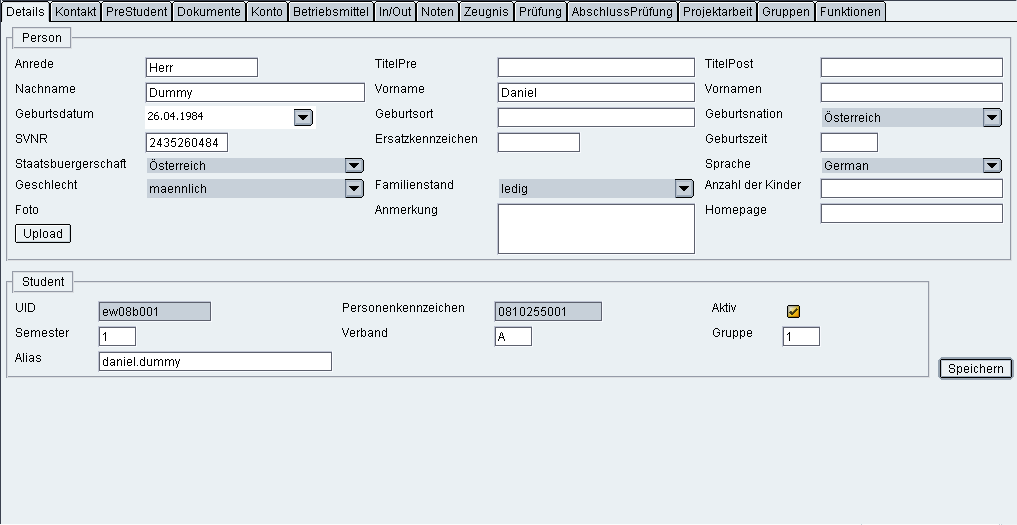
\includegraphics[width=0.75\textwidth]{FAS_Details1.png}
	\caption{Die Karteikarte Details}
	\label{Details1}
\end{figure}
\begin{itemize}
	\item Bereich Person:
	\begin{itemize}
		\item Anrede: Die Anrede der Person findet Verwendung in Ausdrucken wie etwa in Briefk�pfen.
		\item TitelPre: Akademische Titel, die \textbf{vor} dem Name gef�hrt werden. (Um ein hochgestelltes 'a' zu erzeugen halten Sie die <Alt>-Taste gedr�ckt und tippen sie 0170 am Ziffernblick der Tastatur. z.B. f�r Mag�)
		\item TitelPost: Akademische Titel, die \textbf{nach} dem Name gef�hrt werden.
		\item Nachname: Nachname der Person.
		\item Vorname: Vorname der Person.
		\item Vornamen: Weitere Vornamen der Person.
		\item Geburtsdatum: Das Geburtsdatum wird als Entscheidungskriterium f�r die Zusammenlegung von Personendatens�tzen herangezogen, wenn die Sozialversicherung noch nicht eingegeben ist wie es z.B. bei Interessenten vorkommt. Eine Zusammenlegung von Personendatens�tzen wird vorgenommen, damit eine Person nur einmal in der Datenbank abgebildet ist und Redundanzprobleme vermieden werden.
		\item Geburtsort
		\item Geburtsnation
		\item SVNR: Die Sozialversicherungsnummer wird haupts�chlich f�r die BIS-Meldung ben�tigt.
		\item Ersatzkennzeichen: Das Ersatzkennzeichen ist eine Ersatznummer f�r die Sozialversicherungsnummer als �bergangsl�sung bis die Sozialversicherungsnummer vergeben wurde.
		\item Geburtszeit 
		\item Staatsb�rgerschaft: Die Staatsb�rgerschaft wird f�r die BIS-Meldung ben�tigt.
		\item Sprache
		\item Geschlecht 
		\item Familienstand
		\item Anzahl der Kinder
		\item Foto: Die Taste \textsl{Upload} startet einen Dialog zum Einf�gen eines Bildes der Person.
		\item Anmerkung: Hier k�nnen zus�tzliche Informationen eingegeben werden.
		\item Homepage: URL einer Homepage der Person.
	\end{itemize}
	\item Bereich Student:
	\begin{itemize}
		\item UID: Wird bei der Inskription automatisch vergeben, wird vom Personenkennzeichen abgeleitet.
		\item Personenkennzeichen: Eindeutige Identifikationsnummer f�r Studenten. Wird ebenfalls bei der Inskription automatisch vergeben. \\
		Aufbau:
	\begin{itemize}
		\item 2-stellige Jahreszahl der Inskription.
		\item Semesterkennung: 1 f�r WS, 2 f�r SS, 0 f�r Incomingstudenten
		\item 4-stellige Studienkennzahl
		\item 3-stellige laufende Nummer 
	\end{itemize}
		\item Aktiv: Das H�kchen ist standardm��ig gesetzt und gibt an, ob diese Person aktiv studiert und somit ins n�chste Semester vorger�ckt wird oder nicht.
		\item Semester: Ausbildungssemester in dem sich der Student w�hrend des ausgew�hlten Studiensemesters befindet.
		\item Verband: Unterteilung des Ausbildungssemesters.
		\item Gruppe: Unterteilung des Verbands.
		\item Alias: Alternative Emailadresse f�r Studenten. Wird in der Regel automatisch generiert. Regeln: Der Aufbau mu� nach dem Schema \textsl{vorname.nachname} ohne Umlaute erfolgen. Vorname und Nachname m�ssen zumindest je einen Buchstaben lang sein. \textsl{@technikum-wien.at} wird automatisch hinzugef�gt.
	\end{itemize}
\end{itemize}
\newpage
\label{pflichtstamm}
\section{Pflichtfelder}
\begin{figure}
	\centering
	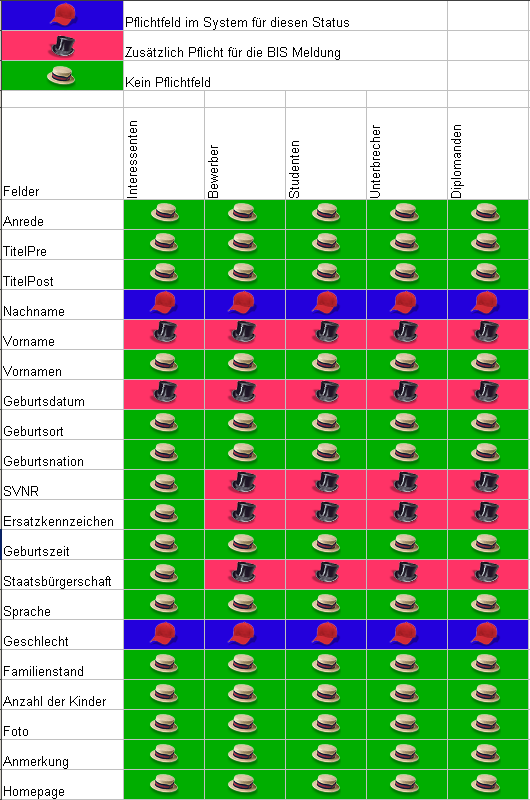
\includegraphics[width=0.75\textwidth]{FAS_Pflichtfelder_Stammdaten.png}
	\caption{Die Pflichtfelder des Karteireiters Stammdaten}
	\label{Bild_Pflichtstamm}
\end{figure}
